\title{Automatic Report Generated by system on runtime of a program with different no of threads}
\author{Bismay Swain}
\documentclass[20pt]{article}
\usepackage{graphicx}
\begin{document}
\maketitle
\clearpage

\begin{figure}
\includegraphics[width=\linewidth]{r1.eps}
\caption{Execution with one Thread}
\label{fig:Scatter1 graph}
\end{figure}
\noindent
This is a scatter plot of time taken for execution v/s Number of
elements when the number of threads created is 1. \\
X-axis holds the number of elements  and
Y-axis displays the time taken correspondingly.
\clearpage

\begin{figure}
\includegraphics[width=\linewidth]{r2.eps}
\caption{2 Threads}
\label{fig:Scatter2 graph}
\end{figure}
\noindent
This is a scatter plot of time taken for execution v/s Number of
elements when the number of threads created is 2. \\
X-axis holds the number of elements  and
Y-axis displays the time taken correspondingly.
\clearpage

\begin{figure}
\includegraphics[width=\linewidth]{r4.eps}
\caption{4 Threads}
\label{fig:Scatter3 graph}
\end{figure}
\noindent
This is a scatter plot of time taken for execution v/s Number of
elements when the number of threads created is 4.
\\
X-axis holds the number of elements  and
Y-axis displays the time taken correspondingly.
\clearpage

\begin{figure}
\includegraphics[width=\linewidth]{r8.eps}
\caption{8 Threads}
\label{fig:Scatter4 graph}
\end{figure}
\noindent
This is a scatter plot of time taken for execution v/s Number of
elements when the number of threads created is 8. \\
X-axis holds the number of elements  and
Y-axis displays the time taken correspondingly.
\clearpage

\begin{figure}
\includegraphics[width=\linewidth]{r16.eps}
\caption{16 Threads}
\label{fig:Scatter5 graph}
\end{figure}
\noindent
This is a scatter plot of time taken for execution v/s Number of
elements when the number of threads created is 16. \\
X-axis holds the number of elements  and
Y-axis displays the time taken correspondingly.
\clearpage

\begin{figure}
\includegraphics[width=\linewidth]{avg1.eps}
\caption{linegraph}
\label{fig:avg graph}
\end{figure}
\noindent
This is a line graph of average time taken for execution v/s Number of
elements. \\
X-axis holds the number of elements  and
Y-axis displays the time taken correspondingly. \\
Different lines represent different no. of threads {1,2,4,8,16}.

\clearpage

\begin{figure}
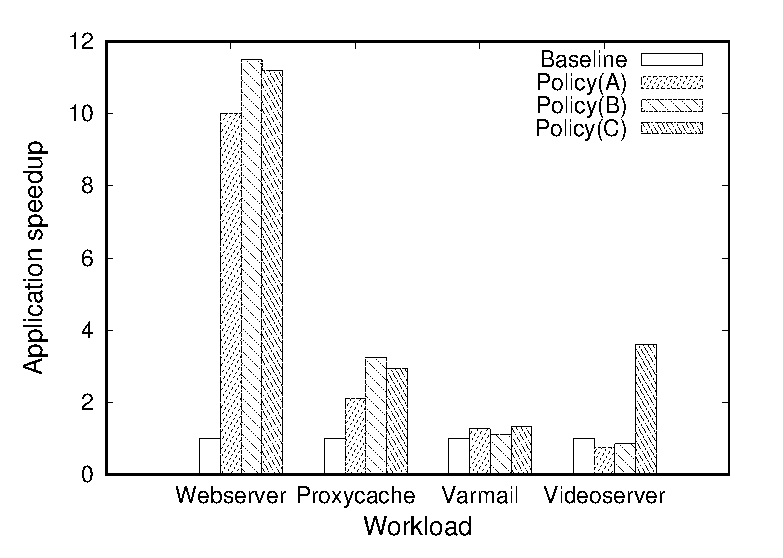
\includegraphics[width=\linewidth]{speedup.eps}
\caption{Bargraph}
\label{fig:Bar graph}
\end{figure}
\noindent
This is a bar graph of average speed for execution w.r.t to the case
with 1 thread v/s Number of elements. \\
X-axis holds the number of elements  and
number of threads {1,2,4,8,16} and Y-axis displays the ratio w.r.t 1
thread.

\clearpage


\begin{figure}
\includegraphics[width=\linewidth]{speedup_err.eps}
\caption{bargraph variance}
\label{fig:Bar graph with error}
\end{figure}
\noindent
This is a bar graph of  speed of execution w.r.t to the case
with 1 thread v/s Number of elements alongside errorbars. \\
X-axis holds the number of elements  and
number of threads {1,2,4,8,16} and Y-axis displays the ratio(time taken)
w.r.t 1 thread and also its variance.

\end{document}
